\documentclass[acmlarge]{acmart}

\setcopyright{acmcopyright}
\copyrightyear{2020}
\acmNumber{4}
\acmMonth{8}

\usepackage{listings}
\usepackage[section]{placeins}
\usepackage{multirow}
\usepackage{pgfplots}

\pgfplotsset{width=7cm,compat=1.8}

\lstdefinelanguage{ocanren}{
keywords={run, conde, fresh, let, in, match, with, when, class, type,
object, method, of, rec, until, while, not, do, done, as, val, inherit,
new, module, sig, deriving, datatype, struct, if, then, else, open, private, virtual, include, success, failure,
true, false},
sensitive=true,
commentstyle=\small\itshape\ttfamily,
keywordstyle=\textbf,%\ttfamily\underline,
identifierstyle=\ttfamily,
basewidth={0.5em,0.5em},
columns=fixed,
mathescape=true,
fontadjust=true,
literate={fun}{{$\lambda$}}1 {->}{{$\to$}}3 {===}{{$\equiv$}}1 {=/=}{{$\not\equiv$}}1 {|>}{{$\triangleright$}}3 {\\/}{{$\vee$}}2 {/\\}{{$\wedge$}}2 {^}{{$\uparrow$}}1,
morecomment=[s]{(*}{*)}
}

\lstset{
language=ocanren
}

\newcommand{\ruleno}[1]{\mbox{[\textsc{#1}]}}

\begin{document}

\title{Fair relational conjunction}

\author{Petr Lozov}
\email{lozov.peter@gmail.com}        

\author{Dmitry Boulytchev}
\email{dboulytchev@math.spbu.ru}    

\affiliation{
  \institution{Saint Petersburg State University}
  \country{Russia}                   
}

\affiliation{
  \institution{JetBrains Research}   
  \country{Russia}                   
}

\begin{abstract}
  Abstract will be here.
\end{abstract}

\begin{CCSXML}
<ccs2012>
<concept>
<concept_id>10011007.10011006.10011008.10011009.10011015</concept_id>
<concept_desc>Software and its engineering~Constraint and logic languages</concept_desc>
<concept_significance>500</concept_significance>
</concept>
</ccs2012>
\end{CCSXML}

\ccsdesc[500]{Software and its engineering~Constraint and logic languages}

\keywords{relational programming, evaluation strategies}

\maketitle

\section{Introduction}

The Reasoned Schemer~\cite{fair:TheReasonedSchemer}

Quine Generation~\cite{fair:quines}

% Проблема несправедливого поведения конъюнкции уже рассматривалась с нескольких разных точек зрения.
The problem of unfair behavior of conjunction has already been examined from several different points of view.

% Одним из аспектов несправедливого поведения конъюнкции является управления приоритетами вычисления независимых ветвей, которые порождает конъюнкция. В оригинальном языке больший приоритет отдается более ранней ветке. Однако существует подход, который позволяет сбалансировать время исполнения. Это делает поведение конъюнкции более справедливым, но чувствительность к порядку конъюнктов сохраняется.
One aspect of the unfair behavior of a conjunction is to prioritize the evaluation of the independent branches that the conjunction generates. In the original \mk, a higher priority is given to an earlier branch. However, there is an approach~\cite{fair:towardsAM} that allows you to balance the time of the evaluation. This makes the conjunction behavior more fair, but the sensitivity to the order of the conjuncts remains.

% Также конъюнкция становится более честной, если детектировать расхождение конъюнктов. Данный подход во время исполнения может обнаружить расхождение конъюкта. В этом случае данные, которые были получены при исполнении конъюнкта стираются. После чего происходит перестановка конъюнктов и продолжается исполнение программы. Данный подход оказывается эффективен на практике. Недостатком является консервативная перестановка конъюнктов, которпя не использует информацию, полученную при вычислении конъюнкта до перестановки.
Also, the conjunction becomes more fair we will detect divergence of conjuncts. This approach~\cite{fair:DivTest} at run time can detect conjunct divergence. In this case, the data that was received during the evaluation of the conjunct is erased. After that there is a rearrangement of the conjuncts and the evaluation of the program continues. This approach is effective in practice. However, the conservative rearrangement of the conjuncts does not use the information obtained when evaluating the conjunct before the rearrangement.

\section{Directed relational conjunction}

% В этом разделе мы рассмотрим реляционный язык miniKanren с классической направленной конъюнкцией, изучим достоинства и недостатки направленной конъюнкции на примерах.
In this section we consider the relational language \mk~ with the classic directed conjunction and demonstrate the advantages and disadvantages of directed conjunction using examples. 

% В языке miniKanren между операциями дизъюнкции и конъюнкции есть существенная разница. Дизъюнкция вычисляет свои аргументы попеременно, что приводит к равномерному вычислению двух дизъюнктов. Такого поведения дизъюнкции достаточно для полного поиска ответов. Конъюнкция же извлекает ответы из первого конъюнкта, на которых вычисляет второй конъюнкт. С одной стороны, такая конъюнкция проста в реализации и позволяет явно задать порядок исполнения конъюнктов. С другой стороны, эта конъюнкция ассиметрична. Более того, она может сходиться при одном порядке конъюнктов, но расходиться при другом. Например, отнонение freeze в зависимости от аргумента либо сходится за один шаг рекурсии, либо расходится. Тогда конъюнкция вида (=== /\ freeze) сходится, но при перестановке конъюнктов мы получаем расхождение. Действительно, в первом случае первый конъюнкт производит ровно один ответ, который противоречит унификации в теле отношения freeze. Во втором случае отношение freeze разойдется и не произведет ни одного ответа и второй конъюнкт вычислен не будет. 
In classic \mk, there is a significant difference between disjunction and conjunction operations. 
The disjunction evaluates its arguments alternately, which leads to the uniform evaluation of two disjuncts. 
This behavior is enough to fully search for answers. 
The conjunction, on the other hand, extracts the answers from the first conjunct and it calculates the second conjunct using this answers.
On the one hand, this conjunction is easy to implement and allows you to explicitly specify the order of evaluation of the conjuncts.
On the other hand, this conjunction is asymmetric. 
Moreover, it can converge in one order of conjuncts, but diverge in another.
For example, relation
\begin{lstlisting}
let rec freeze$^o$ x = x ===  true /\ freeze$^o$ x
\end{lstlisting}
either converges in one recursion step or diverges.
Then conjunction \lstinline{(x === false/\ freeze$^o$ x)} converges, but conjunction with the reverse order of conjuncts \lstinline{(freeze$^o$ x /\ x === false)} diverges.
Indeed, in the first case, the first conjunct produces exactly one answer, which contradicts the unification in the body of the relation \lstinline{freeze$^o$}. In the second case, the relation \lstinline{freeze$^o$} diverges and isn't produce any answer. As a result, the second conjunct will not be evaluated.

% Конечно, данная проблема решается правилом, которому нужно следовать при работе с miniKanren: унификацию нужно ставить самым левым конъюнктом. Но иногда оба конъюнктв являются вызовами отношений. В частности отношение обращения списка revers, которое связывает произвольный список со списком, содержащим элементы в обратном порядке. В этом отношении есть пара конъюнктов append и revers. При таком порядке вызов revers сходится, но при обратном порядке он расходится. Более того при обратном порядке снижается скорость вычисления ответа. 
Of course, this problem can be solved by the rule that must be followed when working with \mk: unification must be the left-most conjunct.
But sometimes both conjuncts are calls of relations.
For instance, the relation \lstinline{revers$^o$} in figure~\ref{fair:lst-reverso}, which associates an arbitrary list with a list containing elements in reverse order.
In this relation we can see a couple of conjuncts: \lstinline{revers$^o$} in line~\ref{fair:reverso-call} and \lstinline{append$^o$} in line~\ref{fair:appendo-call}. In this order, the call \lstinline{(revers$^o$ [1, 2, 3] q)} converges, but in the reverse order it diverges after the answer is found. Moreover, the reverse order decreases the speed of evaluating the answer.

\begin{figure}[h]
\centering
\begin{tabular}{cp{3cm}c}
\begin{lstlisting}[numbers=left,numberstyle=\small]
let rec append$^o$ x y xy =
  (x === [] /\ y === xy) \/
  fresh (e xs xys) (
    x === e : xs /\ 
    xs === e : xys /\ 
    append$^o$ xs y xys)
\end{lstlisting}
& &
\begin{lstlisting}[firstnumber=7,numbers=left,numberstyle=\small,escapeinside={@}{@}]
let rec revers$^o$ x y =
  (x === [] /\ y === []) \/
  fresh (e xs ys) (
    x === e : xs /\ 
@\label{fair:reverso-call}@    revers$^o$ xs ys /\
@\label{fair:appendo-call}@    append$^o$ ys [e] y)
\end{lstlisting}
\end{tabular}

\caption{Relational program to list reversing}
\label{fair:lst-reverso}
\end{figure}

% В то же время, вызов revers при заданном порядке конъюнктов расходится, а при обратном сходится. В результате мы бы хотели разный порядок конъюнктов в зависимости от конкретных аргументов.

At the same time, the call \lstinline{(revers$^o$ q [1, 2, 3])} for a given order of conjuncts diverges, and for the reverse order it converges. As a result, we would like a different order of conjuncts depending on specific arguments.

% В следующих разделах мы предлжожим подход, который будет определять оптимальный порядок автоматически во время исполнения программы.
In the following sections, we propose an approach that will determine the optimal order automatically during program evaluation.
\section{Related work}

Towards a miniKanren with fair search strategies~\cite{fair:towardsAM}

Relational Search via Divergence~\cite{fair:DivTest}
\section{Naive fair conjunction}

\begin{figure}[h!]
\[
set(T, i) =
\left\{
\begin{array}{rl}
(\sigma, i, c_1^i : \ldots : c_n^i : \epsilon), & \mbox{if } T = (\sigma, i, c_1 : \ldots : c_n : \epsilon) \\
(set(T_1, i) \circ set(T_2, i)), & \mbox{if } T = (T_1 \circ T_2)
\end{array}
\right.
\]
\caption{Set semantics}
\label{fair:set-semantics}
\end{figure}

\begin{figure}[h!]
\[\begin{array}{cr}

      {(\sigma, i, \epsilon) \xrightarrow{(\sigma, i)} \circ}  
&     \ruleno{Answer} \\[2mm]
      {(\sigma, i, c_1^0 : \ldots : c_k^0 : \epsilon) \xrightarrow{\circ} (\sigma, i, c_1^N : \ldots : c_k^N : \epsilon)}
&     \ruleno{ConjZero} \\[2mm]
\dfrac{m \not= 0 \qquad (\sigma, i) \vdash c_{i+1} \Rightarrow T \qquad set(m - 1, T) = \bar{T}}
      {(\sigma, i, c_1^0 : \ldots : c_i^0 : c_{i+1}^m : cs) \xrightarrow{\circ} push(c_1^0 : \ldots : c_i^0 : \Box : cs, \bar{T})}
&     \ruleno{ConjUnfold} \\[2mm]
\dfrac{T_1 \xrightarrow{\alpha} \circ}
      {(T_1 \lor T_2) \xrightarrow{\alpha} T_2}
&     \ruleno{Disj} \\[4mm]
\dfrac{T_1 \xrightarrow{\alpha} \bar{T_1}}
      {(T_1 \lor T_2) \xrightarrow{\alpha} (T_2 \lor\bar{T_1})}
&     \ruleno{DisjStep} \\[4mm]
\end{array}\]
\caption{Simple fair semantics}
\label{fair:naive-semantics}
\end{figure}

\begin{figure}
\centering
\begin{tabular}{c}
\begin{lstlisting}
let rec repeat$^o$ e l =
  (l === []) \/
  fresh (ls)
    (l === e : ls /\ 
     repeat$^o$ e ls)
\end{lstlisting}
\end{tabular}

\caption{Relational program to list reversing}
\label{fair:lst-repeato}
\end{figure}

\FloatBarrier


\section{Uniform conjunction by structural recursion}

% В этой секции мы рассмотрим обобщенную семантику \mk с равномерной конъюнкцией, которая определяет глубину раскркутки динамически. Также мы рассмотрим её конкретную реализацию, основонную на структурной рекурсии отношений.
In this section, we consider the generalized semantics of \mk with a uniform conjunction that determines the unfolding depth dynamically. We also consider its specific implementation, which is based on the structural recursion of relations.

% В общем случае мы хотим параметризовать семантику предикатом. Этот предикат принимает вызов в качестве аргумента. Он возвращает истину, если конъюнкт необходимо раскручивать дальше. И возвращает ложь, если необходимо перейти к следующему конъюнкту. Также мы оставим параметр N, определяющий количество раскруток. Он необходим для обработки случая, когда предикат ложен для всех вызовов.
In the general case, we want to parameterize semantics with a unfolding predicate $pred$. This predicate takes a substitution and a call as arguments. He returns \lstinline{true}, if the call needs to be unfolded further. And returns \lstinline{false}, if we need to move on to the next conjunct. We also leave the parameter $N$, which determines the count of unfoldings. It is necessary to handle the case when the predicate $pred$ is false for all calls in leaf.

\begin{figure}[h!]
\[\begin{array}{cr}

      {\inbr{\sigma, i, \epsilon} \xrightarrow{\sigma} \emptyset}  
&     \ruleno{Answer} \\[2mm]
\dfrac{\bigvee_{j=1}^k pred(\sigma, c_j) = \bot}
      {\inbr{\sigma, i, c_1^0 : \ldots : c_k^0 : \epsilon} \xrightarrow{\circ} \inbr{\sigma, i, c_1^N : \ldots : c_k^N : \epsilon}}
&     \ruleno{ConjZero} \\[4mm]
\dfrac{m_{i+1} \not= 0 \qquad \bigvee_{j=1}^k pred(\sigma, c_j) = \bot \qquad (\sigma, i) \vdash c_{i+1} \Rightarrow T \qquad set(m_{i+1} - 1, T) = \bar{T}}
      {\inbr{\sigma, i, c_1^0 : \ldots : c_i^0 : c_{i+1}^{m_{i+1}} : \ldots : c_k^{m_k}} \xrightarrow{\circ} push(c_1^0 : \ldots : c_i^0 : \Box : c_{i+2}^{m_{i+2}} : \ldots : c_k^{m_k}, \bar{T})}
&     \ruleno{ConjUnfold} \\[4mm]
\dfrac{\bigvee_{j=1}^i pred(\sigma, c_j) = \bot \qquad pred(\sigma, c_{i+1}) = \top \qquad (\sigma, i) \vdash c_{i+1} \Rightarrow T \qquad set(m_{i+1} - 1, T) = \bar{T}}
      {\inbr{\sigma, i, c_1^{m_1} : \ldots : c_i^{m_i} : c_{i+1}^{m_{i+1}} : cs} \xrightarrow{\circ} push(c_1^{m_1} : \ldots : c_i^{m_i} : \Box : cs, \bar{T})}
&     \ruleno{ConjUnfoldPred} \\[4mm]
\dfrac{T_1 \xrightarrow{\alpha} \emptyset}
      {(T_1 \lor T_2) \xrightarrow{\alpha} T_2}
&     \ruleno{Disj} \\[4mm]
\dfrac{T_1 \xrightarrow{\alpha} \bar{T_1}}
      {(T_1 \lor T_2) \xrightarrow{\alpha} (T_2 \lor\bar{T_1})}
&     \ruleno{DisjStep} \\[4mm]
\end{array}\]
\caption{Semantics of fair conjunction by structural recursion}
\label{fair:structural-recursion-semantics}
\end{figure}

% Семантика, параметризованная предикатом раскрутки представлена на изображении 10. Так как мы обновляем только поведение конъюнкции, то правила [Answer], [Disj] и [DisjStep]  остаются без изменений. Но за обработку конъюнкций теперь отвечают три обновленных правила. Если предикат истинен хотя бы для одного вызова, то мы применяем правило [ConjUnfoldPred] и раскручиваем самый левый такой вызов и уменьшаем его счетчик. Если предикат ложен на всех вызовах, но есть хотя бы один вызов с ненулевым счетчиком, то мы применяем правило [ConjUnfold] и раскручиваем самый левый такой вызов и уменьшаем его счетчик. Если предикат ложен на всех вызовах и все счетчики равны нулю, то мы применяем правило [ConjZero] и обновляем все счетчики.
The semantics parameterized by the unfolding predicate are shown in Figure~\ref{fair:structural-recursion-semantics}. Since we are updating only conjunction behavior, the rules \rulen{Answer}, \rulen{Disj} and \rulen{DisjStep} remain unchanged. But three updated rules are responsible for handling conjunctions. If the predicate $pred$ is \lstinline{true} for at least one call, then we apply the \rulen{ConjUnfoldPred} rule, which unfolds the left-most such call and decrements its counter. If the predicate $pred$ is \lstinline{false} at all calls, but there is at least one call with a nonzero counter, then we apply the \rulen{ConjUnfold} rule, which unfolds the leftmost such call and decrements its counter. If the predicate is \lstinline{false} at all calls and all the counters are equal to zero, then we apply the \rulen{ConjZero} rule, which set all the counters to $N$.

% В качестве предиката нам необходим критерий, отличающий вызов, который выгодно раскрутить сейчас от вызова, который стоит отложить. Мы предлагаем критерий, который корректно работает на отношениях со структурной рекурсией. У таких отношений есть хотя бы один аргумент, который структурно убывает с каждым шагом рекурсии. Это свойство позволит нам контролировать грубину раскрутки. Предлагаемый критерий состоит в следующем
As a predicate, we need a criterion that distinguishes a call that is profitable to unfold now from a call that is worth deferring. We propose a criterion that works correctly structural recursion relations. Such relations have at least one argument that structurally decreases with each step of the recursion. This property will allow us to control the depth of unfolding. Proposed criterion is as follows

\[
pred(\sigma, F^k(t_1, \ldots, t^k)) = \left\{
\begin{array}{cl}
      & \mbox{if } F^k \mbox{ is structural recursion relation, } \\
\top, & t_i \mbox { is argument of structural recursion, } \\
      & t_i \mbox { is\textquotesingle t fresh variable in } \sigma \\
\bot, & \mbox{otherwise.}
\end{array}
\right.
\]

% Пока хотя бы один аргумент, по которому ведется структурная рекурсия не является свободной переменной, мы продолжаем разворачивать этот вызов. Если все такие аргументы свободны, то в текущей подстановке отношение разойдется, поэтому мы переходим к вычислению следующего вызова. Так как аргументы структурной рекурсии убывают, то за конечное число шагов вычисление либо завершится, либо все аргументы структурной рекурсии станут свободными переменными.
As long as at least one argument along which structural recursion is performed is not a free variable, we continue to unfold this call. If all such arguments are free, then the call will diverge in the current substitution, so we proceed to evaluate the next call. Since the arguments to structural recursion structurally decrease, in a finite number of steps, the evaluation will either complete, or all arguments of structural recursion will become free variables.


\begin{figure}[h!]
\centering
\begin{tabular}{c}
\begin{lstlisting}
let rec append$^o$ x y xy =
  (x === [] /\ y === xy) \/
  fresh (e xs xys) (
    x === e : xs /\ 
    xs === e : xys /\ 
    append$^o$ xs y xys)
\end{lstlisting}
\end{tabular}


\caption{Relational program to append lists}
\label{fair:lst-appendo}
\end{figure}

% Например, отношение appendo является структурно рекурсивным по первому и третьему аргументу. Действительно, вложенный вызов appendo в качестве первого аргумента принимает xs, который является подтермом x. Также в качестве третьего аргумента appendo принимает xys, который является подтермом xy. Если хотя бы один из них --- список фиксированной длины, то отношение сойдется. В противном случае, оба имеют вид: $x = t_1 : \ldots t_n : \alpha$ и $xy = \bar{t}_1 : \ldots \bar{t}_m : \alpha$. Следовательно через max(n, m) шагов оба аргумента станут свободными перееменными. 
For example, the \lstinline{append$^o$} (fig.~\ref{fair:lst-appendo}) relation is structurally recursive in the first and third arguments. Indeed, the nested call \lstinline{append$^o$} takes \lstinline{xs} as its first argument, which is a subterm of \lstinline{x}. Also, \lstinline{append$^o$} takes \lstinline{xys} as the third argument, which is a subterm of \lstinline{xy}. If at least one of them is a fixed-length list, then the relation will converge. Otherwise, $\mbox{\lstinline{x}} = t_1 : \ldots t_n : \alpha_1$ and $\mbox{\lstinline{xy}} = \bar{t}_1 : \ldots \bar{t}_m : \alpha_2$. Therefore, through $max(n, m)$ steps, both arguments become free variables.

% На текущий момент мы работаем над доказательством независимости данной семантики от порядка конъюнктов в случае, когда все отношения являются отношениями со структурной рекурсией.
We are currently working on proving the independence of this semantics from the order of the conjuncts in the case when all relations are relations with structural recursion.

\section{Limitations}
\section{Evaluation}

\begin{figure}[h]
\centering
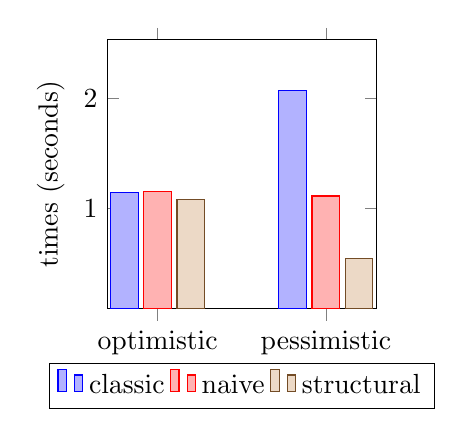
\begin{tikzpicture}
\begin{axis}[
    ybar,
    enlargelimits=0.3,
    width=5cm, height=5cm,
    legend style={at={(0.5,-0.2)},
      anchor=north,legend columns=-1},
    ylabel={times (seconds)},
    symbolic x coords={optimistic, pessimistic},
    xtick=data
    ]
\addplot coordinates {(optimistic,1.142) (pessimistic,2.073)};
\addplot coordinates {(optimistic,1.151) (pessimistic,1.110)};
\addplot coordinates {(optimistic,1.077) (pessimistic,0.542)};
\legend{classic,naive,structural}
\end{axis}
\end{tikzpicture}
  \caption{The results of revers$^o$ evaluation for a list with a length of 90}
  \label{fair:plot-reverso}
\end{figure}

\begin{figure}[h]
\centering
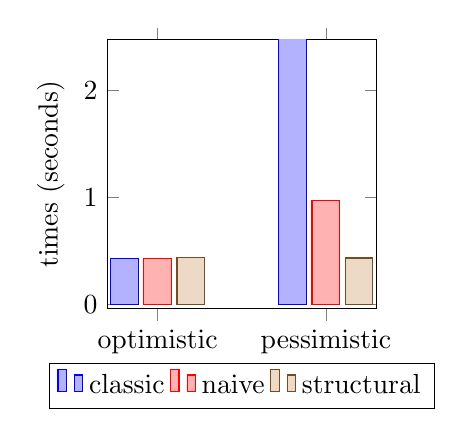
\begin{tikzpicture}
\begin{axis}[
    ybar, ymax = 2,
    enlargelimits=0.3,
    width=5cm, height=5cm,
    legend style={at={(0.5,-0.2)},
      anchor=north,legend columns=-1},
    ylabel={times (seconds)},
    symbolic x coords={optimistic, pessimistic},
    xtick=data
    ]
\addplot coordinates {(optimistic,0.430) (pessimistic,300)};
\addplot coordinates {(optimistic,0.428) (pessimistic,0.969)};
\addplot coordinates {(optimistic,0.433) (pessimistic,0.432)};
\legend{classic,naive,structural}
\end{axis}
\end{tikzpicture}
\caption{The results of sort$^o$ evaluation for a list with a length of 5}
\label{fair:plot-sorto}
\end{figure}

\begin{figure}[h]
\centering
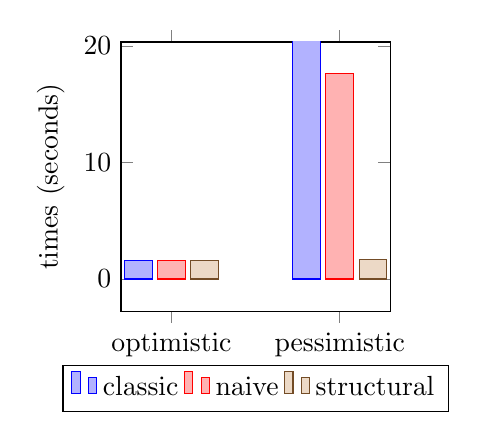
\begin{tikzpicture}
\begin{axis}[
    ybar, ymax = 16,
    enlargelimits=0.3,
    width=5cm, height=5cm,
    legend style={at={(0.5,-0.2)},
      anchor=north,legend columns=-1},
    ylabel={times (seconds)},
    symbolic x coords={optimistic, pessimistic},
    xtick=data
    ]
\addplot coordinates {(optimistic,1.574) (pessimistic,300)};
\addplot coordinates {(optimistic,1.579) (pessimistic,17.604)};
\addplot coordinates {(optimistic,1.585) (pessimistic,1.646)};
\legend{classic,naive,structural}
\end{axis}
\end{tikzpicture}
\caption{The results of ``The Tower of Hanoi'' solver}
\label{fail:plot-hanoi}
\end{figure}

\begin{figure}[h]
\centering
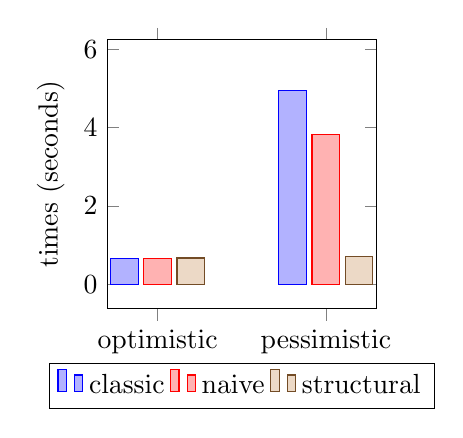
\begin{tikzpicture}
\begin{axis}[
    ybar,
    enlargelimits=0.3,
    width=5cm, height=5cm,
    legend style={at={(0.5,-0.2)},
      anchor=north,legend columns=-1},
    ylabel={times (seconds)},
    symbolic x coords={optimistic, pessimistic},
    xtick=data
    ]
\addplot coordinates {(optimistic,0.669) (pessimistic,4.956)};
\addplot coordinates {(optimistic,0.663) (pessimistic,3.820)};
\addplot coordinates {(optimistic,0.675) (pessimistic,0.712)};
\legend{classic,naive,structural}
\end{axis}
\end{tikzpicture}
\caption{The results of ``Bridge and torch problem'' solver}
\label{fair:plot-bridge}
\end{figure}

\begin{figure}[h]
  \small
  \centering
  \begin{tabular}{ c | c | c | c | c | c | c | c }
    \multirow{2}{*}{relation} & \multirow{2}{*}{size} & 
    \multicolumn{2}{c}{classic conjunction} &
    \multicolumn{2}{c}{naive fair conjunction} &
    \multicolumn{2}{c}{fair conjunction} \\
    \cline{3-8}
    & & optimistic & pessimistic & optimistic & pessimistic & optimistic & pessimistic  \\ 
    \hline
    \multirow{3}{*}{revers$^o$}
                 & 30   & 0.465 & 0.532 & 0.468 & 0.461  & 0.438 & 0.425 \\
                 & 60   & 0.579 & 0.828 & 0.577 & 0.658  & 0.545 & 0.450 \\
                 & 90   & 1.142 & 2.073 & 1.151 & 1.110  & 1.077 & 0.542 \\
    \hline
    \multirow{5}{*}{sort$^o$}
                 & 3    & 0.418 & 0.432 & 0.420 & 0.420  & 0.424 & 0.425 \\
                 & 4    & 0.424 & 3.924 & 0.424 & 0.455  & 0.429 & 0.429 \\
                 & 5    & 0.430 & >300  & 0.428 & 0.969  & 0.433 & 0.432 \\
                 & 6    & 0.434 & >300  & 0.430 & 11.577 & 0.434 & 0.437 \\
                 & 30   & 1.664 & >300  & 1.636 & >300   & 1.723 & 1.751 \\ 
    \hline
    hanoi$^o$    & -    & 1.574 & >300  & 1.579 & 17.604 & 1.585 & 1.646 \\
    \hline
    bridge$^o$   & -    & 0.669 & 4.956 & 0.663 & 3.820 & 0.675 & 0.712    

  \end{tabular}
  \caption{The results of an evaluation: running times of benchmarks in seconds}
  \label{fair:evaluation-table}
\end{figure}
\section{Conclusion}

% В данной работе мы предложили новый подход к исполнению реляционных программ со структурной рекурсией. Данный подход снижает влияние порядка конъюнктов на эффективность исполнения.
In this paper, we proposed a new approach to the execution of relational programs with structural recursion. This approach reduces the impact of conjunct order on performance.

% В дальнейшем мы планируем обобщить предложенный подход для большего класса программ. Также мы планируем формализовать наш подход в системе COQ и доказать, что сходимость вычисления не зависит от порядка конъюнктов.
In the future, we plan to generalize the proposed approach for a larger class of programs. We also plan to formalize our approach in the COQ~\cite{fair:Coq} system and prove that the convergence of the execution does not depend on the order of the conjuncts.

\bibliographystyle{ACM-Reference-Format}
\bibliography{fair-conj}


\end{document}
\endinput

